\documentclass[tikz,border=10pt]{standalone}
\usepackage{tikz}
\usetikzlibrary{positioning, arrows.meta, shapes.geometric}

\begin{document}
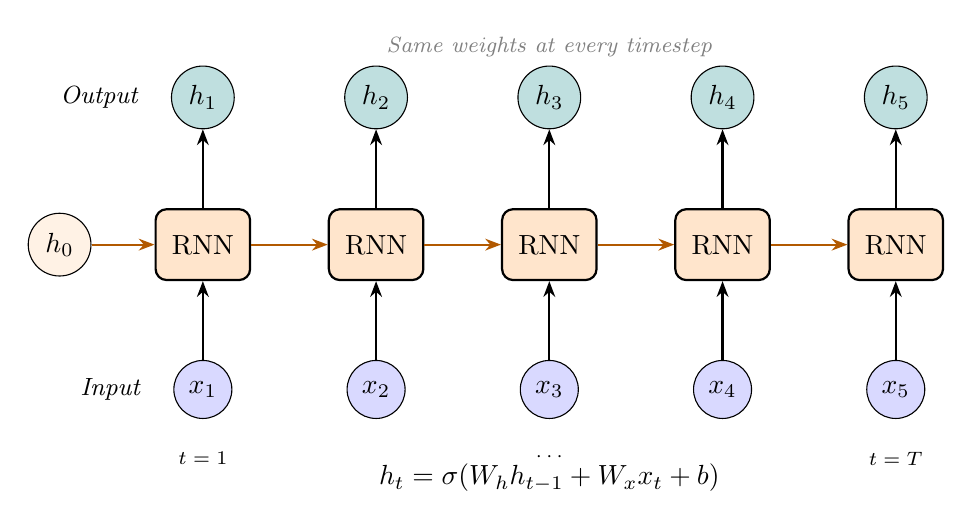
\begin{tikzpicture}[
    node distance=1.8cm,
    cell/.style={rectangle, draw, rounded corners, minimum width=1.2cm, minimum height=0.9cm, thick, fill=orange!20},
    input/.style={circle, draw, minimum size=0.7cm, fill=blue!15},
    output/.style={circle, draw, minimum size=0.7cm, fill=teal!25},
    hidden/.style={circle, draw, minimum size=0.7cm, fill=orange!10},
    arrow/.style={-{Stealth[length=2mm]}, thick},
    harrow/.style={arrow, orange!70!black},
    label/.style={font=\small\itshape}
]

% RNN cells
\foreach \i in {1,...,5} {
    \node[cell] (rnn\i) at (\i*2.2-2.2, 0) {RNN};
}

% Inputs
\foreach \i in {1,...,5} {
    \node[input, below=1cm of rnn\i] (x\i) {$x_{\i}$};
    \draw[arrow] (x\i) -- (rnn\i);
}

% Hidden states (outputs from cells)
\foreach \i in {1,...,5} {
    \node[output, above=1cm of rnn\i] (h\i) {$h_{\i}$};
    \draw[arrow] (rnn\i) -- (h\i);
}

% Horizontal connections (hidden state flow)
\foreach \i [evaluate=\i as \j using int(\i+1)] in {1,...,4} {
    \draw[harrow] (rnn\i) -- (rnn\j);
}

% Initial hidden state
\node[hidden, left=0.8cm of rnn1] (h0) {$h_0$};
\draw[harrow] (h0) -- (rnn1);

% Labels
\node[label, left=0.3cm of x1] {Input};
\node[label, left=0.3cm of h1] {Output};

% Time annotation
\node[below=0.3cm of x1, font=\scriptsize] {$t=1$};
\node[below=0.3cm of x5, font=\scriptsize] {$t=T$};
\node[below=0.3cm of x3, font=\scriptsize] {$\cdots$};

% Equation below
\node[below=2.2cm of rnn3, font=\normalsize] {
    $h_t = \sigma(W_h h_{t-1} + W_x x_t + b)$
};

% Shared weights annotation
\node[above=1.8cm of rnn3, font=\footnotesize\itshape, text=gray] {
    Same weights at every timestep
};

\end{tikzpicture}
\end{document}
